\newpage
\section{Exercise 65:}

Python file: \href{file:./python-scripts/ex65.py}{ex65.py}

\begin{table}[h!]
    \centering
    \begin{tabular}{cccccc}
        \textbf{Class}     & 81~-~\(<\)83 & 83~-~\(<\)85 & 85~-~\(<\)87 & 87~-~\(<\)89                     & 89~-~\(<\)91 \\
        \textbf{Frequency} & 6            & 7            & 17           & 30                               & 43           \\ \hline
        \textbf{Class}     & 91~-~\(<\)93 & 93~-~\(<\)95 & 95~-~\(<\)97 & \multicolumn{2}{c}{97~-~\(<\)99}                \\
        \textbf{Frequency} & 28           & 22           & 13           & \multicolumn{2}{c}{3}                           \\
    \end{tabular}
\end{table}


\subsection{a) Construct a histogram based on relative frequencies.}
\begin{figure}[h!]
    \centering
    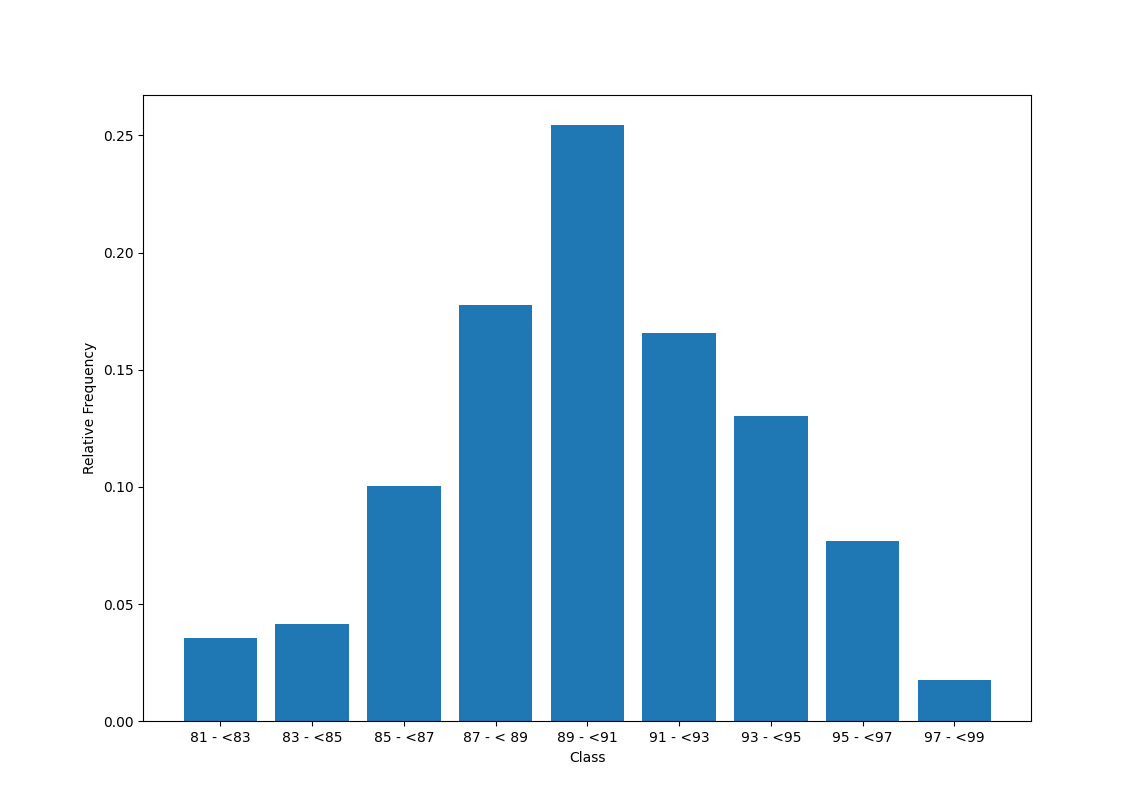
\includegraphics[scale=0.5]{"img/hw1-2a.png"}
    \caption{Histogram based on relative frequencies}
    \label{fig:65a}
\end{figure}

Sum of frequencies: 169
\subsection{b) What proportion of the strength observations are at
    least 85? Less than 95?}

\begin{itemize}
    \item{At least 85\%:}
          \begin{itemize}
              \item Total frequency: \(17+30+43+28+22+13+3=156\)
              \item Proportion: \(\frac{156}{169}=0.9237\)
          \end{itemize}

    \item{Less than 95\%:}
          \begin{itemize}
              \item Total frequency: \(6+7+17+30+43+28+22=\)
              \item Proportion: \(\frac{153}{169}=0.9053\)
          \end{itemize}
\end{itemize}

\subsection{c) Roughly what proportion of the observations are less
    than 90?}
\begin{itemize}
    \item Total frequency: \(6+7+17+30=60\)
    \item Proportion: \(\frac{60}{169}=0.3550\)
\end{itemize}